\documentclass[a4paper]{report}
\usepackage[utf8]{inputenc}
\usepackage{fancyhdr}
\usepackage{graphicx}
\usepackage{mathtools}
\usepackage[bookmarksopen,bookmarksdepth=5]{hyperref}
\usepackage{url}
\usepackage{amsmath}
\usepackage{amssymb}
\usepackage{cite}
\usepackage{listings}
\usepackage[top=30pt,bottom=30pt,left=48pt,right=46pt]{geometry}
\usepackage[fontsize=7pt]{scrextend}

\newcommand{\net}[3]{
\includegraphics[width=0.3\textwidth,height=0.3\textheight,keepaspectratio]{img/#1/#2/#2-1-model.png}
\includegraphics[width=0.3\textwidth,height=0.3\textheight,keepaspectratio]{img/#1/#2/#2-1-history.png}
\includegraphics[width=0.3\textwidth,height=0.3\textheight,keepaspectratio]{img/#1/#2/#2-1-predictions.png}}

\pagestyle{fancy}

\setlength{\headheight}{14pt}

\title{Neurolinguistics Project}
\author{Fabian Klopfer}
\date{March 2019}


\lhead{Fabian Klopfer (956507)}
\rhead{Neurolinguistics}


\begin{document}

\section{Usage}
    \paragraph{Overview:}
    The presented software consists of 3 components:
    \begin{itemize}
        \item A set of functions for parsing the mat-files to python, extracting the desired data from the structure,
            pre-processing
        \item A set of handcrafted neural network models, a common base class for them and the implementation of a Neural
            Architecture search for Regression
        \item A set of functions to visualize the results of the handcrafted networks and the architecture search.
    \end{itemize}
    For additional visualizations of hand-crafted models, navigate in a shell to the path where the weights are saved (should contain the folder 'tensorboard-logs')
    and execute the command " tensorboard --logdir="tensorboard-logs" --port=6006" and access the web interface with your browser at localhost:6006
    \paragraph{Configuration}
    The paths of the data folder and the one to store model weights and metrics to, the electrodes and the frequencies to
    use, training rates and duration can be configured in the file config.py. \\

    \paragraph{Adding a new model} requires the user to inherit from the AbstractNet class and then implement the build
    function and the \_\_init\_\_ function with the provided arguments: \\
    \begin{lstlisting}
def __init__(self, model_out_dir, frequency, electrodes):
    """
    Args:
        model_out_dir: directory to save model to
        frequency: the frequency to be used (shape[1])
        electrodes: the electrodes to be used (shape[0])
    """
    super(DeepDenseNet, self).__init__('WhatsTheNameOfYourModel?', model_out_dir, frequency, electrodes)
    \end{lstlisting}
     The following is a minimal example. For the complete documentation for creating a model see
        \href{https://keras.io/models/model/}{https://keras.io/models/model/} \\
    \begin{lstlisting}
def build(self):
    """
    constructs a model using 1 Dense layer
    Returns:
        the constructed model
    """
    a = Input(self.input_shape)
    x = Flatten()(a)
    b = Dense(1, activation='relu', kernel_initializer='glorot_normal', bias_initializer='zeros', name='1fc2')(x)
    self.model = Model(a, b)
    super().build()
    \end{lstlisting}

    \paragraph{Changing the data format} requires the user to extend preprocessing according to the .mat struct of the
        data. It should however be similar compared to the included preprocessor if data is in the frequency domain,
        e.g. fourier transformed.

\section{Methodology}
The basic workflow was derived from \cite{Tzallas2007AutomaticSD}

\subsection{Pre-Processing}
The provided data contains the coherence spectrum of the fourier transformed recorded EEG and audio stimulus. The
provided labels are comprehension scores between $[0, 1]$ in steps of $0.2$, where each step means an understood word.\\
Below is the covariance matrix of the coherence spectrum and the comprehension scores.
\begin{lstlisting}
Mean Covariance between the Electrode-Audio Coherence spectrum at frequency 5 Hz and the Comprehension Scores
[[1.00992995 0.00153135]
 [0.00153135 0.13221692]]


Mean Covariance between the Electrode-Audio Coherence spectrum at frequency 10 Hz and the Comprehension Scores
[[1.00728738 0.00286027]
 [0.00286027 0.13221692]]
\end{lstlisting}
Thus no pre-processing in terms of signal processing was possible. \\
Data was extracted from the provided .mat-files, filtered to only use user-defined which were determined by cluster
analysis of Dr. Strauß or all electrodes and only a certain frequence or all frequences. The width of the frequency
window was the provided value in Hz $\pm1$, which left 5 channels, if a frequency was specified. The values in the
coherence spectrum were then standardised (z-scores).\\

\subsection{Classification: Neural Architecture Searching for Regression}
Depending on the user input the shape of the input into the neural networks varied between $(n,64,101), \ (n, 64, 5),
\ (n, 6, 101), \ (n, 6, 5)$, thus different network architectures are required to accept different inputs
\cite{tensorflow2015-whitepaper}. This requires the programmer to train at least one model per input shape and in some
cases to adjust the architecture when the results
differ \cite{pmlr-v9-glorot10a}. Architecture search can be a quite time consuming process when done by hand and involves the tuning not only of
the architecture but also hyperparameters like the learning rate. Thus for each input shape every model would have to be
trained a couple of times, which may consum up to several hours per model per input shape \cite{Bengio_2012}. \\

A promising approach to automate architecture search and hyper-parameter tuning is the Neural Architecture Search \cite{DBLP:journals/corr/abs-1806-10282}.
It uses bayesian statistics over the metrics of the composed networks to infer an optimal model configuration.


\subsection{Results}
\begin{tabular}{|c|c|c|c|c|c|}
    MSE & SmallDense & WideDense & DeepDense & MediumConv1D & NAS \\
    5 Hz & 0.1578   & 0.153 & 0.1401 & 0.1390 &  0.126088 \\
    10 Hz &  0.16263 &  0.1542 & 0.14183 & 0.1400 & 0.14444911 \\

\end{tabular}

\section{Appendix: Logs and Plots}
Due to an error of mine (passed 2 Metrics: MAE and MSE, the latter was also the loss function), the MAE is shown as MSE wrongly!
\subsubsection{5 Hz component}

\begin{lstlisting}
    ----------------------------------------------------------------------------------------------------
=========================================Start of Log==============================================
Trained model SmallDenseNet-1.json
Sunday March 31,2019 10:33PM
Dataset dir: C:\Users\Fabi\ownCloud\workspace\uni\7\neuroling\neuroling_project\data\v1
_________________________________________________________________
Layer (type)                 Output Shape              Param #
=================================================================
input_1 (InputLayer)         (None, 64, 5)             0
_________________________________________________________________
flatten_1 (Flatten)          (None, 320)               0
_________________________________________________________________
1fc2 (Dense)                 (None, 1)                 321
=================================================================
Total params: 321
Trainable params: 321
Non-trainable params: 0
_________________________________________________________________
___________Parameters:______________
Batch size    : 128
Epochs       : 10000
Learning rate : 0.02
___________Metrics___________________
Loss          : 0.15788422232073857
MSE      : 0.3429352627324231
=========================================End of Log=================================================
====================================================================================================
----------------------------------------------------------------------------------------------------
\end{lstlisting}
\net{5}{SmallDenseNet}{log}


\begin{lstlisting}
    =========================================Start of Log==============================================
Trained model DeepDenseNet-1.json
Sunday March 31,2019 10:34PM
Dataset dir: C:\Users\Fabi\ownCloud\workspace\uni\7\neuroling\neuroling_project\data\v1
_________________________________________________________________
Layer (type)                 Output Shape              Param #
=================================================================
input_1 (InputLayer)         (None, 64, 5)             0
_________________________________________________________________
flatten_1 (Flatten)          (None, 320)               0
_________________________________________________________________
3fc0 (Dense)                 (None, 128)               41088
_________________________________________________________________
3fc1 (Dense)                 (None, 64)                8256
_________________________________________________________________
3fc2 (Dense)                 (None, 32)                2080
_________________________________________________________________
3fc3 (Dense)                 (None, 16)                528
_________________________________________________________________
3fc4 (Dense)                 (None, 8)                 136
_________________________________________________________________
3fc5 (Dense)                 (None, 4)                 36
_________________________________________________________________
3fc6 (Dense)                 (None, 2)                 10
_________________________________________________________________
3fc7 (Dense)                 (None, 1)                 3
=================================================================
Total params: 52,137
Trainable params: 52,137
Non-trainable params: 0
_________________________________________________________________
___________Parameters:______________
Batch size    : 128
Epochs       : 10000
Learning rate : 0.02
___________Metrics___________________
Loss          : 0.14017007822935293
MSE      : 0.32465702725972745
=========================================End of Log=================================================
====================================================================================================
----------------------------------------------------------------------------------------------------
\end{lstlisting}
\net{5}{DeepDenseNet}{log}


\begin{lstlisting}
    =========================================Start of Log==============================================
Trained model WideDenseNet-1.json
Sunday March 31,2019 10:34PM
Dataset dir: C:\Users\Fabi\ownCloud\workspace\uni\7\neuroling\neuroling_project\data\v1
_________________________________________________________________
Layer (type)                 Output Shape              Param #
=================================================================
input_1 (InputLayer)         (None, 64, 5)             0
_________________________________________________________________
flatten_1 (Flatten)          (None, 320)               0
_________________________________________________________________
0fc0 (Dense)                 (None, 256)               82176
_________________________________________________________________
0fc1 (Dense)                 (None, 64)                16448
_________________________________________________________________
0fc2 (Dense)                 (None, 1)                 65
=================================================================
Total params: 98,689
Trainable params: 98,689
Non-trainable params: 0
_________________________________________________________________
___________Parameters:______________
Batch size    : 128
Epochs       : 10000
Learning rate : 0.02
___________Metrics___________________
Loss          : 0.15357901974220498
MSE      : 0.33593259657049457
=========================================End of Log=================================================
====================================================================================================
----------------------------------------------------------------------------------------------------

\end{lstlisting}
\net{5}{WideDenseNet}{log}

\paragraph{One Layer Dense}
\begin{lstlisting}
    =========================================Start of Log==============================================
Trained model MediumConv1DNet-1.json
Sunday March 31,2019 10:34PM
Dataset dir: C:\Users\Fabi\ownCloud\workspace\uni\7\neuroling\neuroling_project\data\v1
_________________________________________________________________
Layer (type)                 Output Shape              Param #
=================================================================
input_1 (InputLayer)         (None, 64, 5)             0
_________________________________________________________________
0c0 (Conv1D)                 (None, 1, 5)              1605
_________________________________________________________________
flatten_1 (Flatten)          (None, 5)                 0
_________________________________________________________________
0fc0 (Dense)                 (None, 256)               1536
_________________________________________________________________
0fc1 (Dense)                 (None, 64)                16448
_________________________________________________________________
0fc2 (Dense)                 (None, 8)                 520
_________________________________________________________________
0fc3 (Dense)                 (None, 1)                 9
=================================================================
Total params: 20,118
Trainable params: 20,118
Non-trainable params: 0
_________________________________________________________________
___________Parameters:______________
Batch size    : 128
Epochs       : 10000
Learning rate : 0.02
___________Metrics___________________
Loss          : 0.13900083992522577
MSE      : 0.3265306901380506
=========================================End of Log=================================================
====================================================================================================
----------------------------------------------------------------------------------------------------
\end{lstlisting}
\net{5}{MediumConv1DNet}


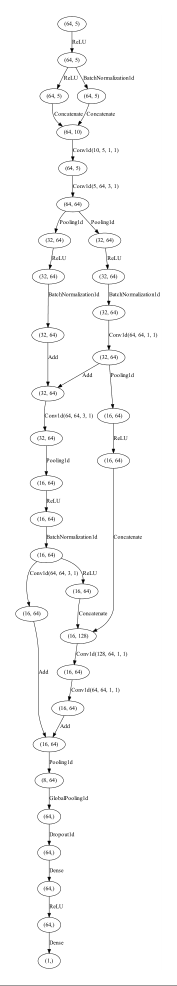
\includegraphics[width=0.3\textwidth,height=0.3\textheight,keepaspectratio]{img/5/NAS/nas-model.png}
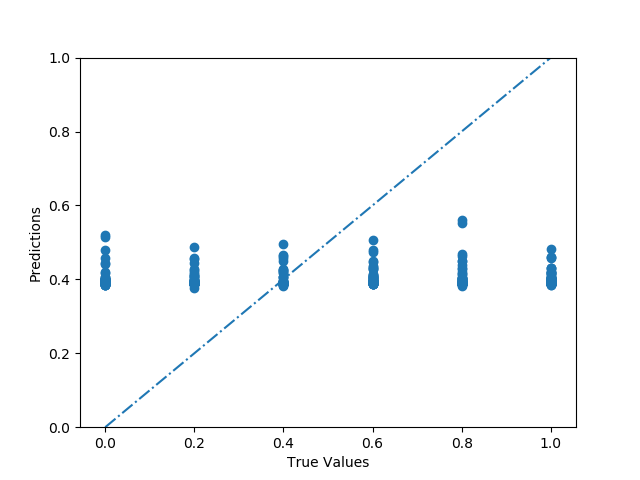
\includegraphics[width=0.3\textwidth,height=0.3\textheight,keepaspectratio]{img/5/NAS/predictions.png}


\subsubsection{10 Hz Component}
\begin{lstlisting}
=========================================Start of Log==============================================
Trained model SmallDenseNet-2.json
Sunday March 31,2019 10:29PM
Dataset dir: C:\Users\Fabi\ownCloud\workspace\uni\7\neuroling\neuroling_project\data\v1
_________________________________________________________________
Layer (type)                 Output Shape              Param #
=================================================================
input_1 (InputLayer)         (None, 64, 5)             0
_________________________________________________________________
flatten_1 (Flatten)          (None, 320)               0
_________________________________________________________________
1fc2 (Dense)                 (None, 1)                 321
=================================================================
Total params: 321
Trainable params: 321
Non-trainable params: 0
_________________________________________________________________
___________Parameters:______________
Batch size    : 128
Epochs       : 10000
Learning rate : 0.02
___________Metrics___________________
Loss          : 0.1626390130016845
MSE      : 0.34865260744370474
=========================================End of Log=================================================
====================================================================================================
----------------------------------------------------------------------------------------------------
\end{lstlisting}
\net{10}{SmallDenseNet}

\begin{lstlisting}

\end{lstlisting}
\net{10}{DeepDenseNet}

\begin{lstlisting}
=========================================Start of Log==============================================
Trained model WideDenseNet-2.json
Sunday March 31,2019 10:30PM
Dataset dir: C:\Users\Fabi\ownCloud\workspace\uni\7\neuroling\neuroling_project\data\v1
_________________________________________________________________
Layer (type)                 Output Shape              Param #
=================================================================
input_1 (InputLayer)         (None, 64, 5)             0
_________________________________________________________________
flatten_1 (Flatten)          (None, 320)               0
_________________________________________________________________
0fc0 (Dense)                 (None, 256)               82176
_________________________________________________________________
0fc1 (Dense)                 (None, 64)                16448
_________________________________________________________________
0fc2 (Dense)                 (None, 1)                 65
=================================================================
Total params: 98,689
Trainable params: 98,689
Non-trainable params: 0
_________________________________________________________________
___________Parameters:______________
Batch size    : 128
Epochs       : 10000
Learning rate : 0.02
___________Metrics___________________
Loss          : 0.154226843073878
MSE      : 0.3378447390705175
=========================================End of Log=================================================
====================================================================================================
----------------------------------------------------------------------------------------------------
\end{lstlisting}
\net{10}{WideDenseNet}

\begin{lstlisting}
=========================================Start of Log==============================================
Trained model MediumConv1DNet-2.json
Sunday March 31,2019 10:30PM
Dataset dir: C:\Users\Fabi\ownCloud\workspace\uni\7\neuroling\neuroling_project\data\v1
_________________________________________________________________
Layer (type)                 Output Shape              Param #
=================================================================
input_1 (InputLayer)         (None, 64, 5)             0
_________________________________________________________________
0c0 (Conv1D)                 (None, 1, 5)              1605
_________________________________________________________________
flatten_1 (Flatten)          (None, 5)                 0
_________________________________________________________________
0fc0 (Dense)                 (None, 256)               1536
_________________________________________________________________
0fc1 (Dense)                 (None, 64)                16448
_________________________________________________________________
0fc2 (Dense)                 (None, 8)                 520
_________________________________________________________________
0fc3 (Dense)                 (None, 1)                 9
=================================================================
Total params: 20,118
Trainable params: 20,118
Non-trainable params: 0
_________________________________________________________________
___________Parameters:______________
Batch size    : 128
Epochs       : 10000
Learning rate : 0.02
___________Metrics___________________
Loss          : 0.14003431685053544
MSE      : 0.32515802600480226
=========================================End of Log=================================================
====================================================================================================
----------------------------------------------------------------------------------------------------
\end{lstlisting}
\net{10}{MediumConv1DNet}

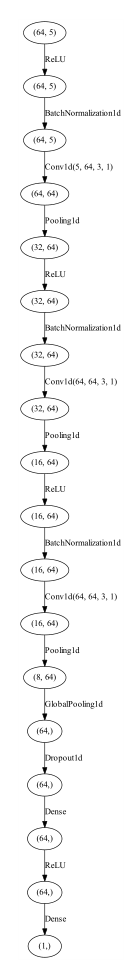
\includegraphics[width=0.3\textwidth,height=0.3\textheight,keepaspectratio]{img/10/NAS/nas_model.png}
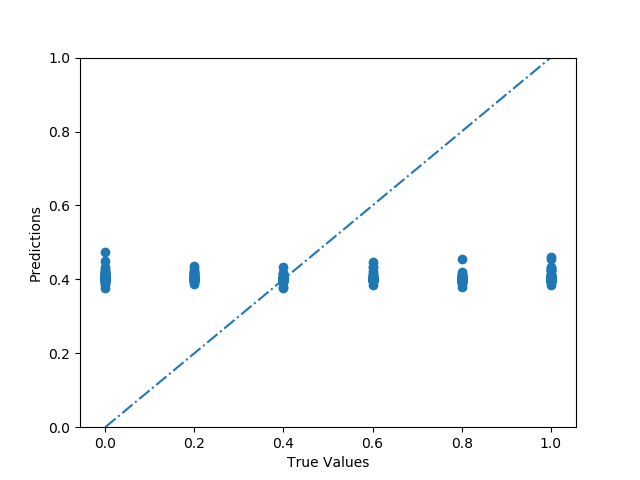
\includegraphics[width=0.3\textwidth,height=0.3\textheight,keepaspectratio]{img/10/NAS/predictions.png}

\bibliographystyle{apalike}
\bibliography{ressources}

\end{document}
